\chapter{Introduction}

\paragraph*{}
This midpoint report aims to highlight the progress of our project throughout the whole semester, with the evaluating criteria being the team's contributions alongside the pace in comparison to the ideal schedule. The ideal project timeline is presented with the Gantt Chart below. (Figure \ref{fig:gantt-chart})

\begin{figure} [H]
    \centering
    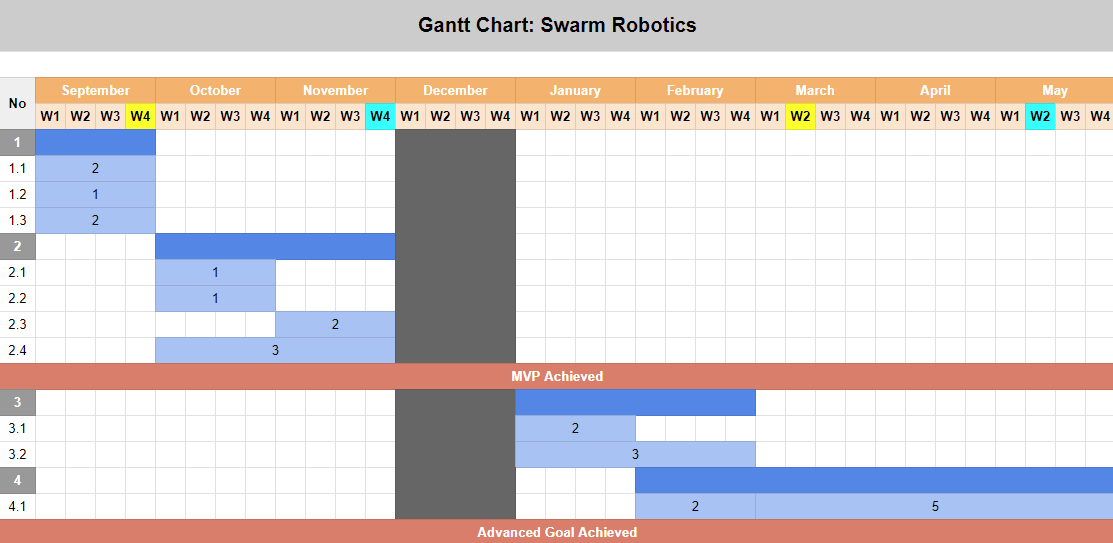
\includegraphics[width=1\linewidth]{assets/images/introduction/gantt_chart.png}
    \caption{Project Gantt Chart}
    \label{fig:gantt-chart}
\end{figure}

\paragraph*{}
Our task allocations can be categorized as two main phases, with the first phase including initial explorations towards fundamental units of understanding necessary for the project completion, that is, \textbf{Communication in the swarm} (Task 1.1), \textbf{Object Detection using Computer Vision} (Task 1.2), and \textbf{Simultaneous Localization and Mapping}. These exploratory endeavors are all completed within \textit{Webots}, a robotic simulation software designed for seamless integration when implemented on actual hardware. The results of these fundamental tasks have all proven satisfactory, as Communication and Object Detection are all successful for the purpose of running a Minimum Viable Prototype simulation. However, Simultaneous Localization and Mapping has been deprioritized due to complications and requirement changes, instead being compensated with \textbf{Localization} (Task 1.3), which has been deemed sufficient for the current simulative implementation.

\paragraph*{}
The second phase entails consolidating the fundamental units into a refined version of simulation, considered as the Minimum Viable Prototype, alongside a few other exploratory tasks on topics such as \textbf{Simple Robot Formation} (Task 2.1), \textbf{Hardware Components} (Task 2.3), as well as a continuation on the deprioritized \textbf{Simultaneous Localization and Mapping} (Task 2.2). Nevertheless, the key highlight of the second iteration will be the \textbf{Combination of the Fundamental Modules in a Single Simulation} (Task 2.4)

\paragraph*{}
The progress of the second phase has also been satisfactory, with the Combined Simulation being completed with an additional bonus of Simple Robot Formation being completed in time to integrate with the Combined Simulation, giving it the ability of navigation. A deeper dive towards each task will be given in the upcoming chapters.

\paragraph*{Current Gantt Chart and Progress:}
\begin{description}
    \item 1.1. Communication -- \textit{Completed}
    \item 1.2. Object Detection using Computer Vision -- \textit{Completed}
    \item 1.3. Localization -- \textit{Completed}
    \item 2.1. Simple Robot Formation -- \textit{Completed}
    \item 2.2. Simultaneous Localization and Mapping -- \textit{In progress}
    \item 2.3. Hardware -- \textit{In progress}
    \item 2.4. Combination of Individual Modules in Simulation -- \textit{Completed}
    \item 3.1. Coordinated gripping -- \textit{To do}
    \item 3.2. Advanced Robot formation -- \textit{To do}
    \item 4.1. Hardware -- \textit{To do}
\end{description}
